\section{Аналитический раздел} \label{analysis}


Аналитический раздел курсовой работы играет ключевую роль в процессе разработки приложения, поскольку он устанавливает основные характеристики системы и выбирает наиболее подходящую модель базы данных. В этой части работы будут изучены различные виды баз данных, их достоинства и недостатки, а также проведен анализ существующих систем управления базами данных. На основе результатов будет выбрана наиболее подходящая модель данных для реализации приложения. Кроме того, в данной секции будут определены акторы системы, будут формализованы данные, а сущности будут представлены отношения между сущностями, что поможет более точно определить требования к приложению и спроектировать его структуру.

\subsection{Требования к приложению}

Так как подача заявки на конференцию, а также модерация может происходить с разных платформ, решено создать серверное приложение, предоставляющее интерфейс для взаимодействия с данными.  Таким образом в дальнейшем для любой платформы можно будет создать клиент, который будет иметь возможность использовать всю функицональность системы.

Система должна поддерживать следующий функционал:
\begin{itemize}[label=---]
		\item возможность авторизации через sso[3] для каждого пользователя;
		\item создание, редактирование, удаление заявки на участие для потенциального докладчика на различные события;
		\item просмотр списка мероприятий для каждого пользователя;
		\item добавление приложений объемом до 10МБ каждое к заявке;
		\item просмотр статуса своих заявок;
		\item возможность взаимодействия докладчика и модератора через комментарии к заявке;
		\item утверждение или отколнения заявки модероатором.
\end{itemize}

\subsection{Анализ существующих решений}

Для анализа существубщих решений были рассмотрены следующие веб-приложения:
\begin{enumerate}
	\item Онтико --- веб-приложение, используемое при проведении конференций highload++, а также некоторых других. Не имеет возможности авторизации через sso, имеет возможность записи на разные конференции.
	\item YaConf --- веб-приложение, используемое при проведении конференций YaConf. Имеется возможность авторизации через аккаунт Яндекса, однако через подать заявку можно только на конференции, проводимые Яндексом.
	\item Jugru --- веб-приложение, используемое для подачи заявок на конференцию cppcon и некоторые другие. Недоступно для мероприятий в России, не имеет входа через sso, есть возможномть записи на разные конференции.
\end{enumerate}

Таким образом, ни одно из существующих решений не удовлетворяет всем требованиям, выдвинутым выше.

\subsection{Пользователи системы}

В приложении выделены следующие роли пользоваталей:
\begin{enumerate}
	\item Потенциальный докладчик (далее просто докладчик) --- пользователь, имеющий возможность авторизоваться, создать заявку на мероприятие, обновить текущую заявку (добавлением комментария к ней), отклонить собственную заявку.. Также докаладчик может посмотреть список доступных для подачи заявок мероприятий и добавить приложений (файл) к своей заявке.
	\item Модерптор --- пользователь, который обладаем правами докладчика, а также может просмтаривать весь список заявок на мероприятий, создавать, редактировать и удалять мероприятия  и одобрять или отклонять заявки.
	\item Администратор --- пользователь, обладающий возможностями модератора, а также возможностью назначать и удалять модераторов.
\end{enumerate}

На рисунке \ref{fig:UseCase} представлена диаграмма использования приложения.

\begin{figure}[h!]
	\centering{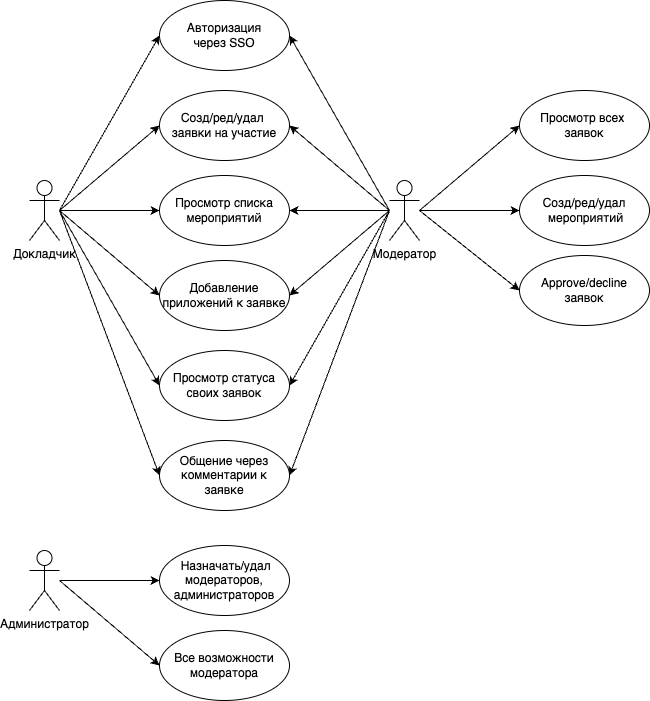
\includegraphics[scale=0.7]{img/use-case.png}}
	\caption{Диаграмма использования приложения}
	\label{fig:UseCase}
\end{figure}

\subsection{Формализация данных}

База данных должна хранить информацию о следующих сущностях:

\begin{itemize}[label=---]
	\item мероприятие;
	\item пользователь;
	\item группа доступов;
	\item заявка;
	\item комментарий к заявке;
	\item приложение (бинарный файл);
	\item мета-информация о приложении.
\end{itemize}


В таблице \ref{decisions} представлены сущности и сведения о них.

\begin{table}[ht!]
	\centering
	\caption{Сущности и сведения о них}
	\label{decisions}
	\begin{tabular}{|p{4.3cm}|p{10.3cm}|}
		\hline
		\textbf{Сущность} & \textbf{Сведения}\\
		\hline 
		\ Мероприятие & Название, описание, дата проведения, продолжительность \\
		\hline 
		\ Пользователь &  Имя, пол, телефон, email-адрес, метка времени первого входа \\
		\hline 
		\ Группа доступов & Название, описание \\
		\hline 
		\ Заяка & Событие, автор, описание, статус, метка времени создания\\
		\hline 
		\ Комментарий к заявке & Текст, событие, автор, время создания \\
		\hline 
		\ Приложение & Бинарные данные \\
		\hline 
		\ Мета-информация о приложении & Имя файла, хеш, размер, метка времени загрузки \\
		\hline
	\end{tabular}
\end{table}

\subsection{Анализ моделей баз данных}

Перед выбором подходящей системы управления базами данных были рассмотрены 3 модели базы данных.

\subsubsection{Объектная модель данных}

Объектные хранилища (Object Stores) представляют собой специализированные хранилища данных, в которых информация хранится в виде объектов. Эти объекты могут содержать не только сами данные, но и дополнительные метаданные, методы и связи с другими объектами. Объектные хранилища широко применяются в различных областях информационных технологий, таких как разработка программного обеспечения, облачные вычисления, хранение данных больших объемов и др.


В данной работе объектная можель данных подходит для хранения приложений (бинарных файлов).  Ключем (путем к файлу) может выступать уникальный идентификатор файла, создаваемый на уровне приложением, а объектом --- сами набор байтов (содержимое файла).

\subsubsection{Иерархическая модель}

Иерархическая модель данных представляет базу данных как древовидную структуру, где объекты различных уровней связаны между собой. Каждый объект может содержать несколько объектов более низкого уровня, устанавливая отношение предка к потомку. Близнецами называются объекты, имеющие общего предка, а в программировании структура дерева также известна как "братья".

Иерархическую модель данных стоит использовать в случаях, когда данные могут быть организованы в виде древовидной структуры с четко выраженными отношениями предок-потомок. Это может быть полезно, когда данные имеют естественную иерархию, например, в организационных структурах, классификациях товаров, семейных деревьях и т. д. Иерархическая модель также подходит для ситуаций, где данные имеют фиксированную структуру и не требуют сложных запросов или изменений в структуре данных. Однако следует учитывать, что иерархическая модель может ограничить гибкость и эффективность обработки данных в случае изменений в их структуре или потребности в сложных запросах. 

В данных формализованных выше отношение предок-потомок имеют только сущности заяка-комментарий, поэтому иерархическая модель не подхожит для применения в данной курсовой работе.

\subsubsection{Реляционная модель}

Реляционная модель данных - основана на понятии математических отношений. В реляционной модели данные и связи представлены в виде таблиц, каждая из которых имеет несколько столбцов с уникальными именами[2]. Основной идеей такой модели является использование ключей для связывания таблиц между собой. Ключ - это уникальный идентификатор, который позволяет однозначно определить каждую строку в таблице. Путем использования ключей можно устанавливать связи между таблицами для получения более сложной информации.

Модель баз данных в форме таблиц обладает рядом преимуществ. Во-первых, при правильном использолвании гарантируется высокая надежность и целостность данных. Во-вторых большое количество самых популарных современных СУБД (Postgres, Oracle, MySql и другие) основаны на реляционной моделе данных.

Однако у этой модели также есть недостатки. Например, она не всегда эффективна при работе с большими объемами информации, так как выполнение сложных запросов может занимать много времени. Кроме того, модель в форме таблиц не всегда подходит для хранения и обработки неструктурированных данных, таких как длинные тексты и бинарные файлы.

В рамках данной работы реляционная модель данных подходит лучше остальным рассмотренных для всех данных кроме сущности <<Приложение>>. Во-первых, все оставшиеся сущности легко представимы в табличной форме, во-вторых использование внешних ключей поможет гарантировать целостность данных.

\subsubsection{Результат анализа моделей баз данных}

Для хранения сущности <<Приложение>> лучше подходит объектная можель содержание файла не находится в каких-либо отношениях с другими сущностями, а значит использование реляционной модели данных не является целесообразным. Также содержимое файла не образует какую-либо иерархию, что говорит о невозможности применения иерархической модели.

Для хранения остальных сущностей реляционная модель подходит лучшим образом, так как данные легко представимы в табличном виде, а также реляционная модель лучше остальных рассмотренных гарантирует целостность данных, что позволит избежать ошибок во время эксплуатации приложения.

\subsection{Выбор объектной базы данных}

При выборе объектной базы данных стоит помнить, что использоваться она будет для хранения приложений (бинарных файлов) объемом до 10МБ. Ниже представлен обзор существующих решений и обоснование выбора базы данных.

\subsubsection{Microsoft Azure Blob Storage}

Microsoft Azure Blob Storage - это облачное хранилище данных, предоставляемое компанией Microsoft в рамках облачного сервиса Azure. Azure Blob Storage предназначено для хранения больших объемов неструктурированных данных, таких как файлы, изображения, видео, аудио, резервные копии, журналы и другие типы информации. Это расширяемое и высокодоступное хранилище, которое обеспечивает надежное хранение данных в облаке с возможностью масштабирования по требованию.

Основной недостаток -- недоступна для использования в России.


\subsubsection{Yandex S3}

Amazon Simple Storage Service (Amazon S3) --- это облачное хранилище данных, предоставляемое Amazon Web Services (AWS). S3 предоставляет возможность хранить и извлекать любое количество данных в Интернете, обеспечивая высокую доступность, надежность и масштабируемость.

Основные характеристики Amazon S3:

\begin{enumerate}
	
	\item доступность и надежность: S3 обеспечивает высокую доступность данных и надежность, гарантируя, что ваши данные будут доступны в любое время;

	\item масштабируемость: S3 позволяет хранить огромные объемы данных без необходимости заботиться о масштабировании инфраструктуры;

	\item управление данными: Вы можете управлять доступом к вашим данным, устанавливать права доступа, шифровать данные и использовать другие функции для обеспечения безопасности информации;

	\item стоимость: Вы платите только за использование, что делает S3 экономически выгодным решением для хранения данных.
\end{enumerate}

Amazon S3 широко используется для хранения резервных копий, статических сайтов, медиафайлов, архивов данных, а также для обработки и анализа больших объемов информации.

Yandex S3 предоставляет совместимый с <<оригинальным>> Amazon S3 программный интерфейс и доступен в России. В современной мирк s3 является де-факто стандартом хранения бинарных файлов.

\subsubsection{Резальтат выбора объектной базы данных}

Для реализации проекта среди 2 рассмотренных вариантов была выбрана база данных Yandex S3, так как она доступна в России и удовлетворяет всем требованиям.


\subsection{Выбор реляционной базы данных}

Ниже представлен обзор существующих решений обоснование выбора базы данных.

\subsubsection{Oracle Database}

Oracle Database - это одна из самых популярных и мощных реляционных баз данных, разработанная компанией Oracle Corporation. Она широко используется в корпоративных средах для хранения и управления данными, обеспечивая высокую производительность, надежность и масштабируемость. Основным недостатком, который делает невохможным применения данной базы данных является отсутствие поддержки этой базы данных выбранным для разработки фреймворком userver.


\subsubsection{MySQL}

MySQL - это одна из самых популярных открытых реляционных баз данных, широко используемая веб-разработчиками и предприятиями для хранения и управления данными. Тем не менее, в рамках данном работы получилось выделить следующие минусы данной системы управления базами данных: 

\begin{enumerate}
	\item ограниченная поддержка даты и времени: MySQL имеет ограниченный набор типов данных для работы с датой и временем, что может вызывать сложности при работе с различными форматами даты и времени или при работе с часовыми поясами;
	\item ограниченные возможности хранения текстовых данных: MySQL имеет ограничения на размер текстовых полей, что может быть проблемой при работе с большими объемами текстовых данных, таких как скрипты выступлений, отправленные через комментарии.
\end{enumerate}
	
Хотя MySQL является мощной и гибкой базой данных, ограниченный набор типов данных может стать препятствием к применению в данном проекте.


\subsubsection{PostgreSQL}

PostgreSQL - это мощная и расширяемая объектно-реляционная система управления базами данных (СУБД), которая широко используется в различных проектах и приложениях. Она является открытой и бесплатной для использования, что делает ее популярным выбором среди разработчиков и организаций. 

PostgreSQL предлагает широкий набор встроенных и сторонних расширений, которые позволяют расширять функциональность базы данных с помощью пользовательских функций, типов данных, операторов и других возможностей. PostgreSQL обеспечивает высокий уровень транзакционной безопасности благодаря поддержке ACID-свойств (атомарность, согласованность, изолированность, долговечность) и механизмам контроля целостности данных.

Из минусов PostgreSQL обычно выделяют отсутствие встроенной возможности шардирования, а также сложность настройки кластера базы данных. В рамках данной работы шардирование не планируется к использованию, а PostgreSQL будет развернута на единичной инсталляции, а не в кластере.

\subsubsection{Результат выбора реляционной базы данных}

В качестве основной базы данных принято использовать PostgreSQL, так как она удовлетворяет заданным требованиям и, кроме того, выбранный для разработки фреймворк userver имеет лучшую поддержку именно этой базы данных.


